\section{Mockup Evaluations}

In total, we had seven subjects come in to evaluate the mockups. We noticed several usability issues with certain features, many of which were subsequently removed. For example, we initially thought we would allow the participants of the competition to vote on their energy goal. The voting interface was a dialog box that was displayed after the user had completed the first login wizard. This confused the subjects in our mockup evaluation, so it was subsequently dropped. Overall, we generated nearly 40 tweaks that needed to be made to the mockups. Many of these tweaks made it in to the final system.

\section{Onboarding Evaluations}

We held two in-lab evaluations; one in April 2010 and one in July 2010.

\subsection{April Evaluation}

We recruited 5 students from the Hale Lehua residence hall at the University of Hawaii at Manoa. Of these students, four were first-year students while one was a senior resident advisor. Of the 5 subjects, only 4 were able to attend both the focus group and the onboarding evaluation. One subject only attended the onboarding evaluation. A summary of results is shown in \autoref{table:april-summary}.

\begin{table}[t]
	\begin{tabular}{| l || p{1cm} | p{1cm} | p{1cm} | p{1cm} | p{1cm} |}
		\hline
		& A & B & C & D & E \\
		\hline
		Points & 51 & 74 & 45 & 74 & 99 \\
		Time taken & 41:39 & 29:49 & 39:15 & 34:24 & 36:11 \\
		First login time taken & 5:26 & 5:06 & 7:08 & 5:40 & 3:01 \\
		Tasks attempted & 12 & 7 & 11 & 15 & 14 \\
		Approved activities & 2 & 5 & 3 & 6 & 7 \\
		Excursions, events, and commitments & 8 & 2 & 5 & 8 & 7 \\
		Rejected activities & 2 & 0 & 3 & 1 & 0 \\
		Allocated raffle ticket(s)? & Yes & Yes & Yes & Yes & Yes \\
		Quests attempted & 5 & 1 & 8 & 1 & 4 \\
		Quests completed & 2 & 1 & 7 & 1 & 3 \\
		\hline
	\end{tabular}
	\caption{Summary of results in April onboarding evaluation}
	\label{table:april-summary}
\end{table}

All five subjects allocated a ticket to the Bubbies gift certificate raffle prize and thus received the prize. Three of the subjects also earned the \textdollar10 bonus for getting to first place on the points scoreboard (60 points or higher).

The following sections will present results related to various components and pages in the site.

\subsubsection{First Login Wizard}

Each of the subjects were able to complete the first login wizard and earn the full 25 points. After each of the subjects completed the first login wizard, we asked them if there were any issues completing it. All of them said that it was very straightforward. However, we observed some minor issues in the process.

Four of the subjects spent a little additional time thinking about what to put in their profile. \autoref{fig:first-login-profile} shows the profile setup phase of the First Login Wizard. The main issue was the ``about'' field. Some subjects wondered out loud if they could type in anything into that field. The about field's label confused one subject, who thought it was a yes or no question.

\begin{figure}[t]
  \center
  \includegraphics[width=0.5\textwidth]{images/first-login-profile.eps}
  \caption{First Login Wizard profile setup}
  \label{fig:first-login-profile}
\end{figure}

This version of the system also had an explicit Facebook setup step in the First Login Wizard before the profile step. This was because we wished to asynchronously post news and events to the walls of players. All five of the subjects had a Facebook account, but only three signed up as part of the First Login Wizard. One player connected their Facebook account later and mentioned that they were unsure as to what their Facebook information would be used for. After they watched the introduction video, they understood why they might want to connect with Facebook.  The fifth player wanted to complete the Facebook activity in the Smart Grid Game, but could not remember their password.

\subsubsection{Quests}

Only two out of the five subjects saw the quest bar right away. One subject did not see the quest bar until about 12 minutes into the evaluation. The last two subjects did not see the quest bar until about 20 minutes into the evaluation. These two subjects saw the ``Win the \textdollar10 bonus'' and the Bubbies Gift Certificate quests, so the possibility of winning something caught their eye. A possible reason why subjects may have missed the quest bar is because it looks identical in style to the other boxes in the page. An example of the quest bar is shown in \autoref{fig:quest-bar}.

\begin{figure}[t]
    \center
    \includegraphics[width=0.5\textwidth]{images/quest-bar.eps}
    \caption{The Quest Bar on an Activity's page}
    \label{fig:quest-bar}
\end{figure}

\autoref{table:april-quest} is a table of the quests each subject attempted and how long they took to complete the task. Most of the subjects accepted a quest and then got distracted by other things. The main exception was subject C, who read the quest descriptions, accepted the quest, and carried out its instructions immediately. Subject B also completed their lone quest relatively quickly (they watched a 4 minute long video), but the ``Win the \textdollar10 bonus'' quest is more open ended than the others.

\begin{table}[t]
	\begin{tabular}{| l || l | l | l | l | l |}
		\hline
		Quest & A & B & C & D & E \\
		\hline
		Get the Fully Committed Badge & Incomplete & & & & Incomplete \\
		Win the \textdollar10 Bonus & Incomplete & 6:53 & Incomplete & & 8:44 \\
		Learn About Energy & & 9:15 & & 13:14 &\\
		Make a Commitment & & 0:50 & & 9:35 & \\
		Win a Bubbies Gift Certificate & 0:16 & & 0:13 & 2:56 & \\
		Get a Grip on Energy Use & & & 1:17 & & \\
		Get Social & Incomplete & & 4:42 & & \\
		Sign Up For An Excursion & 6:53 & & 0:39 & & \\
		Sign Up For An Event & & & 2:04 & & \\
		\hline
	\end{tabular}
	\caption{Quests performed by users in the April evaluation}
	\label{table:april-quest}
\end{table}

While the visibility of the quest bar is a significant issue, we also have the issue of users failing to carry out the quest once completed. Subject C mentioned that putting the important parts of the quest descriptioin in bold would make it easier to complete quests. Another possibility would be to use images in the description to illustrate what users are supposed to see and/or click on. Other issues with quests were that one subject almost canceled a quest they were reading about and that most of the quests involve the ``Get Nutz'' section of the website.

\subsubsection{Home Page}

\begin{figure}[t]
    \center
    \includegraphics[width=0.5\textwidth]{images/home-april.eps}
    \caption{Layout of the six top level pages on the home page}
    \label{fig:home-page-april}
\end{figure}

\autoref{fig:home-page-april} shows the home page of the website. Two of the subjects went to the ``Go Low'' page first after completing the first login wizard. The icon for this page was in the top left corner of the home page content and these users both reported that it was the first page they saw. Subject C went to the profile page first with the intent of making changes to their profile after watching the introduction video. One subject accepted the ``Make a commitment'' quest on the home page, but they then went to the prizes page because they were interested in what they could win. The last subject went to the ``Get Nutz'' page first because they were specifically looking for the Smart Grid Game and thought that is where it would be.

\subsubsection{Go Low}

\begin{figure}[t]
    \center
    \includegraphics[width=0.5\textwidth]{images/energy-april.eps}
    \caption{The Go Low Page}
    \label{fig:energy-page-april}
\end{figure}

\autoref{fig:energy-page-april} shows the ``Go Low'' page of the website as it was in April 2011. Because it was the first page listed in the home page, two users came here with little information about what is going on in the page. Subjects that came here before completing the ``Power and Energy'' and ``Energy Intuition'' tasks were confused as to what is going on in this section. One of these subjects asked about the energy goals and who sets them while another became confused by the energy calculator. The calculator was designed to calculate how many hours you need to \emph{not} do something in order to reduce your energy usage. A subject using the energy calculator compared the amount of time one needs to not play Xbox versus the amount of time one needs to not play Wii and came to the conclusion that the Wii uses more power because the number was higher. This is not the case; since the Wii uses less power, you must reduce your playing for a longer period of time. Those subjects that came here first eventually left the page by selecting an activity in the ``How can we meet our energy goal'' list of activities.

The ``Learn about your energy use'' activity brought subjects back to this page later on. This activity asked users to check if they are over or under their energy goal, by how much, and what they can do to reduce their energy usage. One subject fully understood what was going on and completed the task efficiently. Another subject (who went to the ``Go Low'' page early on) came back to do the activity and also completed it. The activity included an image of the power gauge that users were supposed to look at on the ``Go Low'' page. This caused one subject to use the information from that static image to complete the activity.

After the evaluation, the subjects did mention that they had a better understanding of what was going on in this page after playing the Smart Grid game for a while.

\subsubsection{Get Nutz}

\begin{table}[t]
	\begin{tabular}{| l || p{1cm} | p{1cm} | p{1cm} | p{1cm} | p{1cm} |}
		\hline
		Activity & A & B & C & D & E \\
		\hline
		Power and Energy & 3:13 & 3:02 & \bf{3:16} & 3:01 & 2:21 \\
    Energy Intuition & \bf{3:53} & 3:52 & \bf{4:25} & \bf{4:12} & 3:34 \\
    Like Kukui Cup on Facebook & & 1:03 & 2:33 & 2:41 & \\
    Share Kukui Cup on Facebook & & & 1:16 & 1:10 & \\
    Examine Your Lounge's Energy Use & & & 1:11 & 1:09 & \\
    Configure Computer to Sleep After Inactivity & & 1:04 & & &  \\
    Trash is Treasure & & 5:29 & & & \bf{4:21}* \\
    Climate Change & & & & & 4:17 \\
    Wind Energy & & & & & 2:43 \\
    Solar Energy & & & & 3:35 & \\
		\hline
	\end{tabular}
	\caption{Activity items completed during the April evaluation}
	\label{table:april-activities}
\end{table}

Three out of the five subjects that came here clicked on the ``Intro video'' item in the grid even though they had already completed it as part of the first login sequence. These users went through the video for a little bit to make sure that it was the same video that they already saw.

All of the subjects that viewed the grid expressed some initial confusion as to what is going on in the Smart Grid Game. One subject mentioned that the introduction video did not explain how to play the game at all. A few subjects clicked on the question marks hoping that there would be some response. At this point, the question marks did nothing, which left the subjects even more confused. However, once they clicked on a number (which is an unlocked task and represents the amount of points the task is worth), the subjects began to understand how the Smart Grid Game works. One subject even mentioned that the numbers turn to the name of the task as they complete them.

When completing tasks that involve videos, only two of the subjects went back to watch the video when they did not know the answer. The other three tried to guess the answers to the questions without going back to the videos. The two subjects who went back to watch the videos to answer the question correctly were the two highest point getters in this evaluation.

For the most part, subjects had few issues with actually completing tasks. As part of submitting the task, we included an ``additional comments'' section that was to be used to provide feedback about the task from the user to the administrators of the competition. Three of the subjects took the time to input text into the box for every single task. While this section is optional, the text does not explicitly say so. Another interesting outcome was that one user declined to sign up for events or excursions that they were unable to make in real life. The event/excursion dates were based around the time of the evaluation. This probably is not an issue, but it was interesting given that signing up for events and excursions award points and the events and excursions were not actually going to occur.

\begin{figure}[t]
    \center
    \includegraphics[width=0.5\textwidth]{images/april-screenshot-upload.eps}
    \caption{Upload a Screenshot Instructions}
    \label{fig:april-screenshot-upload}
\end{figure}

Three of the activities (Share Kukui Cup Link on Facebook, Like Kukui Cup on Facebook, and Configure Computer to Sleep After Inactivity) required subjects to take a screenshot and upload it. Instructions were displayed as part of the activity description like in \autoref{fig:april-screenshot-upload}. Some subjects were able to take the screenshot quickly without looking at the instructions. However, subjects who were more used to Windows PCs had difficulty figuring out how to take the picture. There was not much we could do in terms of changing the evaluation due to limitations in our available hardware, but we decided to use screenshots sparingly and only when needed. For example, liking the Kukui Cup on Facebook can be verified simply by asking subjects for their Facebook name.

What happens after submitting responses for a task was another major issue. At the time of the evaluation, we displayed a red box near the top of the page whenever a submission is rejected by administrators. However, the red box only shows up once before disappearing. Out of the five subjects, only one of them caught the box even once and did something about it. Another subject eventually found out that one of their tasks was rejected from their profile page. The subject clicked on the ``rejected'' link and saw that the administrators left a response for them. This subject mentioned that it was good that the administrators provided feedback and that they could read it. However, they did not go back and try to complete the task, even though a button was provided for the subject to click on and try again.

Subjects were also confused by the rotating scoreboards on the ``Get Nutz'' page. One subject, who was trying to get the number one score, was confused that they were number one on one scoreboard, but later checked and found themselves lower. In this case, the subject was number one on their floor, but not overall. Another subject noted that the scoreboard rotated too quickly.

There was a bug in our evaluation where subjects could not access certain activities in the website. This occurred because the system failed to select a question for certain activities. This bug affected the subjects depending on what their database id was, so some subjects were able to access activities that other were not. Subject B in particular encountered the error more than once. The solar energy video was also not intended to be shown, but subject D found it and completed it.

\subsubsection{Prizes Page}

Other than the one subject who came here to see what they could win, the subjects primarily came here as part of the Bubbies gift certificate quest. The subjects understood how the raffle works and how tickets can be allocated. The only issue was that one subject was concerned that adding or removing tickets would decrease their point total.

\subsubsection{Discussion}

Overall, the sessions were a success. The subjects uncovered several usability issues, many of which we would not have thought of on our own. The primary issues that came out of the evaluation were the missed rejection notifications, the quest bar, and having the Go Low page listed first on the home page. As a result of these evaluations, we created a notification component that made the rejected notifications more ``sticky'', changed the color of the quest bar, and changed the order of the pages on the home page so that the Get Nutz page is first.

We were provided with positive feedback regarding the game. When asked if individuals would recommend it to their friends, all of the subjects said that they think their friends would be in to it. Some found the points aspect ``addicting'' while others thought the near-real time power meter and energy displays were ``cool''. Some of the subjects were disappointed that they would not be able to participate in the actual competition (because it will be held for the first-year students in the following year).

\subsubsection{Focus Group}

Four participants were able to make it to the focus group. Subjects were asked about their attitudes to energy conservation and about their experience with the system. They also provided valuable suggestions that can be applied to the design of content for Makahiki and ways we can market the events and excursions.

\subsection{July Evaluation}

We recruited five different participants from the Hale Lehua residence hall who were available over the summer. Again, four of the participants were first year students and one was a resident advisor. Four subjects were able to make it to both the onboarding evaluation and the focus group, while the fifth could not make it to the focus group. \autoref{table:july-summary} is a summary of the results in the July evaluation.

\begin{table}[t]
	\begin{tabular}{| l || p{1cm} | p{1cm} | p{1cm} | p{1cm} | p{1cm} |}
		\hline
		& A & B & C & D & E \\
		\hline
		Points & 113 & 83 & 101 & 74 & 72 \\
    Time taken & 39:35 & 41:05 & 36:57 & 37:35 & 49:04 \\
    First login time taken & 3:10 & 3:59 & 3:40 & 4:00 & 3:34 \\
    Tasks attempted & 13 & 10 & 16 & 7 & 14 \\
    Approved activities & 9 & 6 & 8 & 3 & 4 \\
    Excursions, events, and commitments & 4 & 4 & 7 & 4 & 7 \\
    Rejected activities & 0 & 0 & 0 & 0 & 3 \\
    Allocated raffle ticket(s)? & No & Yes & Yes & Yes & No \\
    Quests attempted & 3 & 7 & 8 & 6 & 1 \\
    Quests completed & 3 & 3 & 8 & 3 & 1 \\
		\hline
	\end{tabular}
	\caption{Summary of results in July onboarding evaluation}
	\label{table:july-summary}
\end{table}

\subsubsection{Changes}

We made several changes going into the July evaluation. The first login wizard used to contain a Facebook Connect step that informed users we would be posting to their wall. We decided to scrap the idea and instead incorporated the Facebook Connect button into the profile step. The ``about'' field in the profile step was also removed, since that information was not displayed elsewhere in the system.

We changed the color of the quest bar. Previously, the quest bar looked very similar to other ``widgets'' in the system, which may have caused users to ignore it. The color of the quest bar was changed to a black background with white text, so it is now unique compared to other user interface elements in the system.

We knew we needed to improve the video/answer question workflow in the SGG. First, we added an explicit cancel button and text that tells the user they can close the window and review the video if they need to. Second, when a submitted answer is rejected, we display a message to the user just below the quest bar that is persisted as the user navigates around the site. In addition, answers that are rejected also appear as a modal dialog box that has to be closed before the subject can continue using the site. These boxes can contain multiple notifications, so users do not see more than one at a time.

We also added a video to the SGG called ``Secrets of the Kukui Cup Masters''. This video provides ``strategies'' that can be used to win the game. These strategies provide a little explanation to some of the components of the game. In addition to the video, a new quest was added that guides the user to this video. The videos on solar energy and wind energy were removed. Liking the Kukui Cup on Facebook was changed to ask for a Facebook name instead of a screenshot.

\subsubsection{First Login Wizard}

Everyone got through the first login wizard in 4 minutes or less. It seems that the profile step did hang people up in the previous evaluation. We can say that the first login wizard takes about 5 minutes in the introduction. Also, the subjects did not customize their profile and stuck to the default profile name and profile image. None of the subjects used their picture from Facebook, even though some of them logged into Facebook later on in the evaluation. During the actual competition, 48 users signed in to Facebook to use their image. All of these users linked to Facebook in the first login wizard.

\subsubsection{Quests}

\begin{table}[t]
	\begin{tabular}{| l || l | l | l | l | l |}
		\hline
		& A & B & C & D & E \\
		\hline
		Secrets of the Kukui Cup Masters & 9:13 & Opt-out & 0:00 & 0:00 & \\
    Make a Commitment & 0:30 & & 13:05 & Incomplete & 22:37 \\
    Win the \textdollar10 bonus & 2:49 & 0:00 & 0:00 & 9:15 & \\
    Sign Up For An Event & & 5:55 & 0:55 & & \\
    Sign Up For An Excursion & & Incomplete & 0:21 & 0:37 & \\
    Win a Bubbies Gift Certificate & & 0:07 & 1:13 & & \\
    Get Social & & Opt-out & & Incomplete & \\
    Get the Fully Committed Badge & & Incomplete & 13:30 & & \\
		\hline
	\end{tabular}
	\caption{Quests completed by subjects in the July evaluation}
	\label{table:july-quests}
\end{table}

\autoref{table:july-quests} is a summary of the quests attempted and completed by the subjects. Subjects in this evaluation saw the quest bar within 5 minutes of finishing the first login wizard, so changing the color of it was very successful. There were still a few instances where someone did not know they needed to accept the quest. It might be good to have a simple introductory quest that shows a user how to  add a quest. That quest would be completed as soon as they add it. We would need a predicate for this quest to check if the user has ever completed a quest before.

We had an issue with the way the quests were set up. For a few of the quests, the unlock condition for the quest was true even if the subject already completed the steps required for the quest. The quests in particular were the Secrets of the Kukui Cup Master's quest and the Win the \textdollar10 Bonus quest. A few subjects saw the quest complete as soon as they added it. Subject B was reading about the Secrets quest and realized they had already done it, so they were confused. We instructed them to opt out of the quest because they had already completed it.

Other issues were that subject E was a little confused when they looked at their achievements in their profile. The subject knew that they completed the quest, but was confused as to why they weren't awarded points for it. After subject B opted out of the Secrets quest, they opted out of the Get Social quest since they did not use Facebook.

\subsubsection{Smart Grid Game/Actions}

\autoref{table:july-activities} is a summary of the activities attempted by users. The times recorded represent the first time they attempted the activity. Bolded items were rejected. Starred items were rejected but later resubmitted and approved.

\begin{table}[t]
	\begin{tabular}{| l || p{1cm} | p{1cm} | p{1cm} | p{1cm} | p{1cm} |}
		\hline
		Activity & A & B & C & D & E \\
		\hline
		Power and Energy & 3:05 & 3:13 & 2:45 & 4:38 & \bf{3:37} \\
    Secrets of the Kukui Cup Masters & 5:26 & 5:48 & \bf{4:34}* & 5:05 & 5:43 \\
    Energy Intuition & 4:13 & 4:13 & & & \bf{3:42} \\
    Like Kukui Cup on Facebook & 1:10 & & 0:57 & & 1:28 \\
    Share Kukui Cup on Facebook & 2:19 & & 2:05 & & \\
    Examine Your Lounge's Energy Use & 3:07 & 3:36 & 1:40 & & 6:28 \\
    Configure Computer to Sleep After Inactivity & 3:27 & & & & \bf{3:52} \\
    Trash is Treasure & & 5:00 & 3:00 & & \\
    Take a survey & 3:29 & & & 4:41 & \\
		\hline
	\end{tabular}
	\caption{Activity items completed during the July evaluation}
	\label{table:july-activities}
\end{table}

Overall, our success rate with these activities were very high compared to the previous evaluation. The issue that came up during subject E's evaluation was that they received a notification for being rejected for one activity right after they submitted a response for another one. The subject thought the rejection notice was for the one they just did (Energy Intuition) when the rejection notice was referring to the ``Power and Energy'' activity they did previously. As for the ``Configure Computer to Sleep'' activity, the screenshot did not have the necessary information and the subject declined to resubmit.

Subjects were also a lot more likely to close the question window if they didn't remember the answer to a question in the video. During the previous evaluation, the subjects tried to guess and got it wrong. Having the cancel button and the text that says they can close the window and review the material was a major addition and got subjects to correctly answer questions. The addition of a modal dialog when activities are rejected also worked very well for subject C, who was able to resubmit their response when they go the answer to a question wrong.

We were also able to implement surveys for the first time. Subjects were able to complete the surveys without much issue. However, we were not satisfied with the implementation of the survey type and decided to remove the feature from the system. Instead, surveys in the beta evaluation and production system were handled using SurveyGizmo, a third party service for creating surveys. Users in the actual competition provided their name in the survey so that we could determine who to award points to.

\subsubsection{Onboarding Evaluation Summary}

\autoref{table:onboarding-summary} compares the average results of the April evaluation to the July evaluation.

\begin{table}[t]
	\begin{tabular}{| l || l | l |}
		\hline
		& April & July \\
		\hline
		Points & 68.6 & 88.6 \\
		Time taken & 36:16 & 40:51 \\
    First login time taken & 5:16 & 3:40 \\
    Actions attempted & 11.8 & 12 \\
    Approved activities & 4.6 & 6 \\
    Excursions, events, and commitments & 6 & 5.2 \\
    Rejected activities & 1.2 & 0.6 \\
    Allocated raffle ticket(s)? & 5/5 & 3/5 \\
    Quests attempted & 3.8 & 5 \\
    Quests completed & 2.8 & 3.6 \\
		\hline
	\end{tabular}
	\caption{Average results of the April and July evaluations.}
	\label{table:onboarding-summary}
\end{table}

Although we gave the subjects in the second evaluation a little more time, their point total went up by 20 points. This is 0.0424 points per minute in the April evaluation and 0.0534 points per minute in the July evaluation, so subjects in the July evaluation were more productive than the subjects in the April evaluation. Subjects in the evaluation also took less time to complete the first login wizard, possibly due in part to the removal of the optional ``about'' text field in the profile setup. Subjects also attempted and completed more quests in the July evaluation, meaning the change in color for the quest bar made it more visible to subjects.

% Note: need to summarize actions for April.
The number of actions attempted by the subjects were about equal despite the increased time taken and reduced first login wizard time. However, in terms of activities, subjects in the July evaluation had more of their activities approved and half the number of rejections. In fact, all of the rejections in the July evaluation were from one subject, while three subject had submissions rejected in the April evaluation.

% \subsubsection{Focus Group}
% 
% Again, 4 of our participants were able to make it to the focus group. We again asked about their attitudes toward energy conservation and their experience with the system. We also dove deeper into their life in the residence halls and what they like or do not like about living there. This was to get additional insight into the residence hall ``community'' and how often they interact with each other.

\subsection{Beta Evaluation}

The beta evaluation started on August 11th, 2011 to August 17th, 2011. We had 4 teams take part in the test, each with 5 members. Three of the four teams were fielded by local companies and organizations, while the fourth involved friends and family.

\subsubsection{Changes}

Because of the increased length of this evaluation, we needed a lot more content in the system. In addition to new videos, we created advanced actions that were more involved. Advanced actions included creating a poem related to sustainability, making a video, or writing a song. We also wanted suggestions on how we could improve the competition, so an action in the Smart Grid Game was created to suggest ways to promote the competition. We also had prizes to give away to participants, so that content was added to the prizes page.

\subsubsection{Results}

\begin{table}[t]
	\begin{tabular}{| l || l | l | l | l | l | l | l | l |}
		\hline
		Subject & Points & First Login & \multicolumn{2}{c}{Quests} & \multicolumn{2}{c}{Commitments} & \multicolumn{2}{c|}{Activities} \\
		& & & completed & attempted & completed & attempted & completed & attempted \\
		\hline
    A & 1103 & 3:45 & 3 & 3 & 5 & 10 & 24 & 25 \\
    B & 1078 & 4:55 & 3 & 3 & 5 & 10 & 25 & 25 \\
    C & 1062 & 4:43 & 0 & 0 & 10 & 15 & 20 & 21 \\
    D & 1054 & 8:38 & 2 & 2 & 15 & 17 & 22 & 22 \\
    E & 1053 & 3:29 & 5 & 5 & 15 & 20 & 21 & 21 \\
    F & 993 & 3:23 & 1 & 1 & 4 & 9 & 24 & 24 \\
    G & 953 & 6:25 & 3 & 3 & 0 & 5 & 21 & 21 \\
    H & 943 & 3:45 & 1 & 1 & 0 & 5 & 21 & 21 \\
    I & 930 & 6:40 & 4 & 4 & 5 & 10 & 19 & 19 \\
    J & 925 & 5:48 & 4 & 5 & 5 & 9 & 18 & 18 \\
    K & 903 & 6:09 & 1 & 2 & 4 & 9 & 16 & 16 \\
    L & 878 & 5:29 & 2 & 2 & 0 & 5 & 16 & 16 \\
    M & 858 & 8:40 & 3 & 3 & 0 & 5 & 15 & 16 \\
    N & 855 & 6:12 & 1 & 1 & 0 & 5 & 14 & 14 \\
    O & 773 & 9:02 & 0 & 0 & 4 & 9 & 5 & 10 \\
    P & 760 & 5:00 & 0 & 0 & 0 & 5 & 7 & 8 \\
    Q & 689 & 5:24 & 0 & 0 & 0 & 2 & 3 & 3 \\
    R & 665 & 2:57 & 0 & 0 & 0 & 0 & 0 & 0 \\
		\hline
	\end{tabular}
	\caption{Summary of results in the beta evaluation.}
	\label{table:beta-summary}
\end{table}

\autoref{table:beta-summary} is a summary of the results of the beta evaluation. Of the 20 users entered into the system, 18 logged in to the system at least once. On average, the users that logged in averaged 915.28 points and they each completed 1.8 quests, 4 commitments, and 16.2 activities.

\subsubsection{Issues}

One major issue that came up in the beta evaluation was that the website did not perform well on Internet Explorer. In particular, the buttons on the landing page were rendered in a way that made them inaccessible in earlier versions of IE. These participants were using laptops provided to them by their workplace, so they were unable to install browsers on their computers. For the purposes of the evaluation, this was solved using Google Chrome Frame~\cite{google-chrome-frame}, which allows early versions of IE to use Google Chrome as a rendering engine. This also did not require administrator permission to install, so these users could use it and be able to navigate around the site. 

While the above issue is unlikely to occur in the residence halls, we do need to make sure the front page works for the most popular browsers and also be able to detect if a user is using an outdated version of that browser. We fixed the rendering issue on the landing page and implemented a browser check that checks the user's browser on the landing page. If they are using an outdated browser, they will be notified that the system does not support it.

We also encountered a bug with commitments where individuals were losing points when they added a commitment. This bug was fixed and points were added back in, but this also caused us to think of a way to detect this in the future. We later implemented a points transaction log that gets created whenever a user adds or removes points. We can use this log to detect anomalies in the point values of individuals and fix them when needed.

Finally, a subject was confused when they already had points going into the first login wizard. This occurred because the individual started the evaluation a day late and daily energy goal game already awarded points. While this was not a bug, we decided to only award daily energy goal game points to individuals who were already logged in to the system.

\subsubsection{Post Beta Survey}

At the end of the beta evaluation period, we sent out the post-beta survey. A summary of their responses are in \autoref{appendix:beta-survey}.The first question was about what aspects they liked about the beta test. Many liked the gamification and learning aspects of the system. When asked what aspects they liked least, some reported the lack of content and the lack of reminders. We also asked the participants what their primary motivators and de-motivators were. Some again reported the lack of content (some blew through the content in the first month) and the lack of real energy data as de-motivators, but many found the points and prizes to be a great motivator.

We also asked them for suggestions for improving the competition. We got some feedback about the canopy. The participants in this test were not motivated to participate in the canopy because there were no points to be awarded. We also received suggestions for a few tweaks to the interface as well as tips on getting people motivated to participate in the competition. Finally, we asked for additional comments.

\section{Production Results}

The inaugural Quest for the Kukui Cup was held at the University of Hawaii at Manoa from October 17th, 2011 to November 6th, 2011. The competition involved the four Hale Aloha residence halls, housing 1,013 first year students and their resident advisors. Of these 1,013 students, 418 of them logged in to the website at least once.

During round one of the competition, we came up with the referral bonus, which is another way we tried to get more people to log in to the site. This was added to the first login wizard as an additional step. In order to get the referral bonus, the user had to enter the email address of a participant in the system. Then, the user had to earn 30 points before the user and the participant that referred them got 20 points each. This was developed and deployed to the live site in 4 days. Within minutes of the update, a new user went through the process and added a referring user.

\subsection{Issues}
While the referral bonus was tested and pushed out relatively quickly, it was also the source of a major bug that resulted in awarding thousands of points to two individuals. In comparison, the highest score was about 1,000 at that point in time. The bug in the code was fixed and pushed out a few hours after the incident occurred. We also encountered an issue where some people could ``double submit'' a form, meaning that they could send an additional request to the server when they should only have been able to send one. It mainly caused issues in events and commitments, where a signup bonus may be assessed multiple times. This was difficult to track down and fix. We periodically inspected the points transaction logs and the commitment/event signups and corrected the user's points value when needed.

\subsection{Results}

\begin{table}[t]
	\begin{tabular}{| l || l | l | l | l | l |}
		\hline
		Page & Total time & Average Time & Percent of total \\
		\hline
		Home & 84.43 & 0.20 & 9.82\% \\
    Activities & 550.24 & 1.33 & 64.03\% \\
    Energy & 87.52 & 0.21 & 10.18\% \\
    Prizes & 73.50 & 0.18 & 8.55\% \\
    Canopy & 7.46 & 0.18* & 0.87\% \\
    Help & 8.62 & 0.021 & 1.01\% \\
		\hline
	\end{tabular}
	\caption{Hours spent on the website during the 2011 Kukui Cup.}
	\label{table:prod-summary}
\end{table}

\autoref{table:prod-summary} outlines the results of the competition. While the average time was calculated based on the total number of participants, note that the canopy was based on the 42 individuals that were admitted to the canopy in round 3. Overall, 850 hours were spent on the web site. As expected, most of the time was spent on the activities, energy, and prizes page. During the prior evaluations, these were the pages we focused on. However, the canopy was not widely used even among the individuals who were admitted. We believe the canopy is a great idea, but we need to invest more time designing it and presenting it to users in evaluations. Out of the evaluations we performed, it was clearly the least tested component as we had it available only for a few days during the beta evaluation.

A survey to gather the opinions of participants was added during the third round. 42 of the participants completed the survey. When asked ``What did you like about the website?'' in a free response question, 25 of them said ``ease of use''. When asked what they found confusing, 13 of them said ``nothing''. 11 of them again said ``nothing'' when asked what they would change about the website. While the participants that made it to the third round are invested in the competition, it is nonetheless encouraging that users found the system easy to use. Of course, the feedback of the other individuals will be investigated as we further evolve the system.

We also had a few statements for users that were evaluated using a likert scale. Those results are shown in \autoref{table:prod-likert} as percentages of respondents who marked each statement. Overall, the system performed very well during the 2011 Kukui Cup. 

\begin{table}[t]
	\begin{tabular}{| p{6cm} || l | l | l | l | l |}
		\hline
		& Strongly Disagree & Disagree & Neutral & Agree & Strongly Agree \\
		\hline
		It was easy to find what I was looking for on the website & 4.7 & 2.3 & 4.7 & 32.6 & 55.8 \\
		The website was responsive & 4.7 & 2.3 & 2.3 & 44.2 & 46.5 \\
		The website provided adequate help in teaching me how to play & 2.3 & 2.3 & 2.3 & 37.2 & 55.8 \\
		I understood how to play & 2.3 & 2.3 & 0 & 27.9 & 67.4 \\
		\hline
	\end{tabular}
	\caption{Statements evaluated on a likert scale during the 2011 Kukui Cup.}
	\label{table:prod-likert}
\end{table}